\documentclass[12pt,a4paper]{article}
\usepackage{pgf}
% \usepackage[condensed,math]{kurier}
% \usepackage[T1]{fontenc}
\usepackage{svg}
\usepackage{tikz}
\usepackage{stanli}
\usepackage{afterpage}
\usepackage{multirow}
\usepackage{subfig}
\usepackage{pgfpages}
\usepackage{listings}
\usepackage{biblatex} %Imports biblatex package
\usepackage{rotating}
\usepackage{bookmark}
\usepackage{hyperref}

\usepackage{xcolor}
\usepackage{svg}
\definecolor{codegreen}{rgb}{0,0.6,0}
\definecolor{codegray}{rgb}{0.5,0.5,0.5}
\definecolor{codepurple}{rgb}{0.58,0,0.82}
\definecolor{backcolour}{rgb}{0.95,0.95,0.92}

\lstdefinestyle{mystyle}{
    backgroundcolor=\color{backcolour},   
    commentstyle=\color{codegreen},
    keywordstyle=\color{magenta},
    numberstyle=\tiny\color{codegray},
    stringstyle=\color{codepurple},
    basicstyle=\ttfamily\footnotesize,
    breakatwhitespace=false,         
    breaklines=true,                 
    captionpos=b,                    
    keepspaces=true,                 
    numbers=left,                    
    numbersep=5pt,                  
    showspaces=false,                
    showstringspaces=false,
    showtabs=false,                  
    tabsize=2
}

\lstset{style=mystyle}

%\usepackage{times}


\pgfpagesdeclarelayout{boxed}
{
	\edef\pgfpageoptionborder{0pt}
}
{
	\pgfpagesphysicalpageoptions
	{%
		logical pages=1,%
	}
	\pgfpageslogicalpageoptions{1}
	{
		border code=\pgfsetlinewidth{2pt}\pgfstroke,%
		border shrink=\pgfpageoptionborder,%
		resized width=.9\pgfphysicalwidth,%
		resized height=.9\pgfphysicalheight,%
		center=\pgfpoint{.5\pgfphysicalwidth}{.5\pgfphysicalheight}%
	}%
}

\pgfpagesuselayout{boxed}


% Language setting
% Replace `english' with e.g. `spanish' to change the document language
\usepackage[english]{babel}
\usepackage{csvsimple}
% Set page size and margins
% Replace `letterpaper' with `a4paper' for UK/EU standard size
\usepackage[a4paper,top=2cm,bottom=1.5cm,left=1.5cm,right=1.5cm]{geometry}

% Useful packages
\usepackage{amsmath}
\usepackage{graphicx}

\title{}
\author{}
\date{}

\bibliography{refs.bib}

\begin{document}

\newcommand{\subf}[2]{%
    {\small\begin{tabular}[t]{@{}c@{}}
                #1 \\#2
            \end{tabular}}%
}

\begin{titlepage}
    \begin{center}
        \vspace*{3cm}

        \Huge
        \textbf{Massive Parallel Cracker}

        \vspace{0.3cm}
        \Huge
        MD5

        \vspace{0.8cm}
        \large

        %INSTRUCTED BY: MRS. A.A.S.KAUSHLYA


        \vspace{0.5cm}
        \LARGE


        \vspace{1.5cm}

        \textbf{}
        %\includegraphics[width=0.8\textwidth]{./Images/model.png}

        \vfill



        \vspace{0.8cm}



        \Large




    \end{center}
    \Large
    \begin{tabbing}
        \hspace*{1em}\= \hspace*{8em} \= \kill % set the tabbings
        \> Name:\>  \textbf{Matteo Ielacqua} \\
        \> ID:\>  \textbf{839241} \\
    \end{tabbing}

\end{titlepage}


\section{Introduction}
Distributed crack is an MPI, MultiThreaded and GPU enabled software that let the user to try different password combination on a single hash using all the power of the distributed computing. The program is thinked as an extensible example of how implement a distributed hash calculator alongside various string generators.

\subsection{Hashing algorithm}
An hashing algorithm is a function that takes as input some bytes, usually divided in blocks of fixed length, and returns an array of bytes of fixed length. Examples of those functions are MD4/5 (a.k.a Message Digests algorithms), SHA-1/2/256/512. Those functions are used in databases in order to maintain privacy, suppose we have a web application that takes username and password in order to authenticate user, if we are interested in avoid to store those data as clear string then hashing is a good way to obfscate those data. That's why the existence of tools like jhontheripper, hydra and distributedcrack shall be taken in consideration, also if we use an hash to obfuscate a password if the input is not long enough is relatively easy to "invert" the function by trying all the different ascii combinations. Nowadays there are strict policy around password due to those tools, you need to supply a 12 char password with some special character for that password, prevent inversion by bruteforcing. Unfortunately this length will grow in time, since the release of new hardware will let hackers to use much more "muscles" in order to calculate the original password. As always hacking something is just a matter of time.

\subsection{MD5}
MD5 is a fast, efficient but not secure hashing algorithm. All hashing algorithm are designed with the intent to provide a specific and stable \(i.e of constant length\) output for all kind of inputs, but since they lack a mathematical proof of their behaviour we are satisfied to assume they work until the contrary is proven. That is the case for MD5, which a collision was found in 2004, and since then it is not considered a secure hashing algorithm, hovewer due to its simplicity it is still used in some applications like message authentication in non safety critical protocols.

\section{The application}
Develop an application to parallelize in hashing algorithm is the target of many hackaton, many applications surrounding the SHA-1 and SHA-256 algorithms were written, usually combining both GPU and CPU load. In this istance my objective was quite simple: write an application that can calculate a password stored as MD5 with both dictionary and bruteforce attack.

\subsection{Tools and languages used}
The project is divided in 2 parts: the libraries and the core. Under the libraries there are 2 implementation of the MD5 hashing algorithm, one for the cpu with also a string generator written both in C,  and the other for the gpu written in CUDA with a compatible string generator. The core program in written in Rust, a modern and memory safe programming language, with the MPI functions exported using bindgen and FFI (Foreign Function Interface) of Rust, and Rayon as a framework to develop the parallel evaluation of the strings to be hashed.


\subsection{Brief description of the libraries}
The libraries hold the implementation of the MD5 algorithm and the string generator for the bruteforce mode.

\subsubsection{CPU Version}
In the CPU version it is only necessary to supply an arbitrary string to the function 
\begin{lstlisting}
    void md5String(char *input, uint8_t *result);
\end{lstlisting}

The computed result of 16 bytes will be returned. This implementation of the MD5 algorithm works as intended by the literature, so a string of characters is shuffled (using different bitwise operations) with a magic table that provide the constant used in the hashing algorithm. Each step of the algorithm is performed on 512 bit of input, that are padded when the remained characters are less than this measure.

\begin{lstlisting}
    void md5Step(uint32_t *buffer, uint32_t *input){
        uint32_t AA = buffer[0];
        uint32_t BB = buffer[1];
        uint32_t CC = buffer[2];
        uint32_t DD = buffer[3];
        uint32_t E;
        unsigned int j;
        for(unsigned int i = 0; i < 64; ++i){
            switch(i / 16){
                case 0:
                    E = F(BB, CC, DD);
                    j = i;
                    break;
                case 1:
                    E = G(BB, CC, DD);
                    j = ((i * 5) + 1) % 16;
                    break;
                case 2:
                    E = H(BB, CC, DD);
                    j = ((i * 3) + 5) % 16;
                    break;
                default:
                    E = I(BB, CC, DD);
                    j = (i * 7) % 16;
                    break;
            }
            uint32_t temp = DD;
            DD = CC;
            CC = BB;
            BB = BB + rotateLeft(AA + E + K[i] + input[j], S[i]);
            AA = temp;
        }
        buffer[0] += AA;
        buffer[1] += BB;
        buffer[2] += CC;
        buffer[3] += DD;
    }
\end{lstlisting}

The string generator instead is a container of all possible permutation of a string of visible characters in utf8 so in the range $ [!(33) , tilde (126)]$. 

\begin{lstlisting}
    struct SequenceGeneratorCtx new_seq_generator(uint8_t base_len);
    void seq_gen_next_sequence(struct SequenceGeneratorCtx* ctx);
    void seq_gen_skip_to(struct SequenceGeneratorCtx* ctx,size_t address);
\end{lstlisting}

The generator start from a base length of the string and treats every further combination as an address (or offset) from this base length. This behaviour guarantee that the user can also skip to a certain combination specifing just the address, that will be calculated using a modified version of the combinatorial search proposed by Donald Knuth \cite{artcp1}. 

\begin{lstlisting}
    void seq_gen_skip_to(struct SequenceGeneratorCtx* ctx,uint64_t address)
{
    int div = maxCharint - minCharInt;
    int q = address;
    int r = 0;
    int it = 0;
    while (q > 0)
    {
        r = q % div;
        q /= div;
        if (it == ctx->current_len)
        {
            shift_buffer(ctx->buffer, ctx->current_len, 1); 
            ctx->current_len++;
            ctx->buffer[0] = minCharInt;
        }
        ctx->buffer[ctx->current_len - it - 1] = (char)(r + minCharInt);
        it++;
    }
}

\end{lstlisting}

The importance of this algorithm will be explained in the next subsection about the core and communication between nodes. 

\subsubsection{GPU Version}
The GPU version of the MD5 algorithm works more or less like the CPU version, it is implemented in CUDA, the real difference between the general C library and this implementation resides in the management of memory and the support to the 2 different modes of attack.

\begin{lstlisting}
    struct Md5TransformResult{
    char* data;
    size_t size;
}; 
struct Md5BruterResult{
    char data[33];
    bool found;
};
struct Md5TransformResult md5_gpu(char* data, uint8_t * sizes, size_t array_size, int maxthreads);
struct Md5BruterResult md5_bruter(size_t start_address, size_t end_address, const char* target_md5, int maxthreads,int base_str_len);
\end{lstlisting}

In fact the first function let the user trasform a flat sequence of bytes that should represent the strings in input in a vector of data, each with a corresponding size and obtain then a flat sequence of digested MD5. Instead, in the brute version, the user shall pass a start and an end address, that correspond to the offsets of the string generator in the C version, useful for brute forcing, if the target md5 is found is returned. One may ask: why then not apply the same technique in the trasform version, so check in the GPU when a target is found instead of return the vector with MD5 digest? The response is that the user should allocate enough space to retain the strings to process, this is a huge bottleneck, if instead of compare just a single target the user compare multiple targets the effect of this bottleneck is reduced, also if a second transfer is required from the GPU to the CPU.

\subsection{Brief description of the core}
The core implements the communication between nodes, that are divided in generator node (usually the root) and worker nodes. 

\subsubsection{The Dictionary / Chunked mode}
In dictionary attack mode there are 2 nodes:
\begin{itemize}
    \item The generator node: this hold the control of the dictionary file and send splitted chunks of data to each of the worker node 
    \item The worker node: this request a chunk whenever is free to compute, and tell the root when a result is found.
\end{itemize} 

The quantity of data involved in each message is decided by the user through the chunk size option. Upon start the master node will wait for a request from any node, when a request is received the master answer with a data communication , each data communication will involve 2 messages, the first is a vector of unsigned bytes with length equal to the chunk size, the second is the actual data. The communication is done in 2 distinct messages so that the client can allocate enough buffer to contain the actual data to be trasformed. 

\begin{figure}
    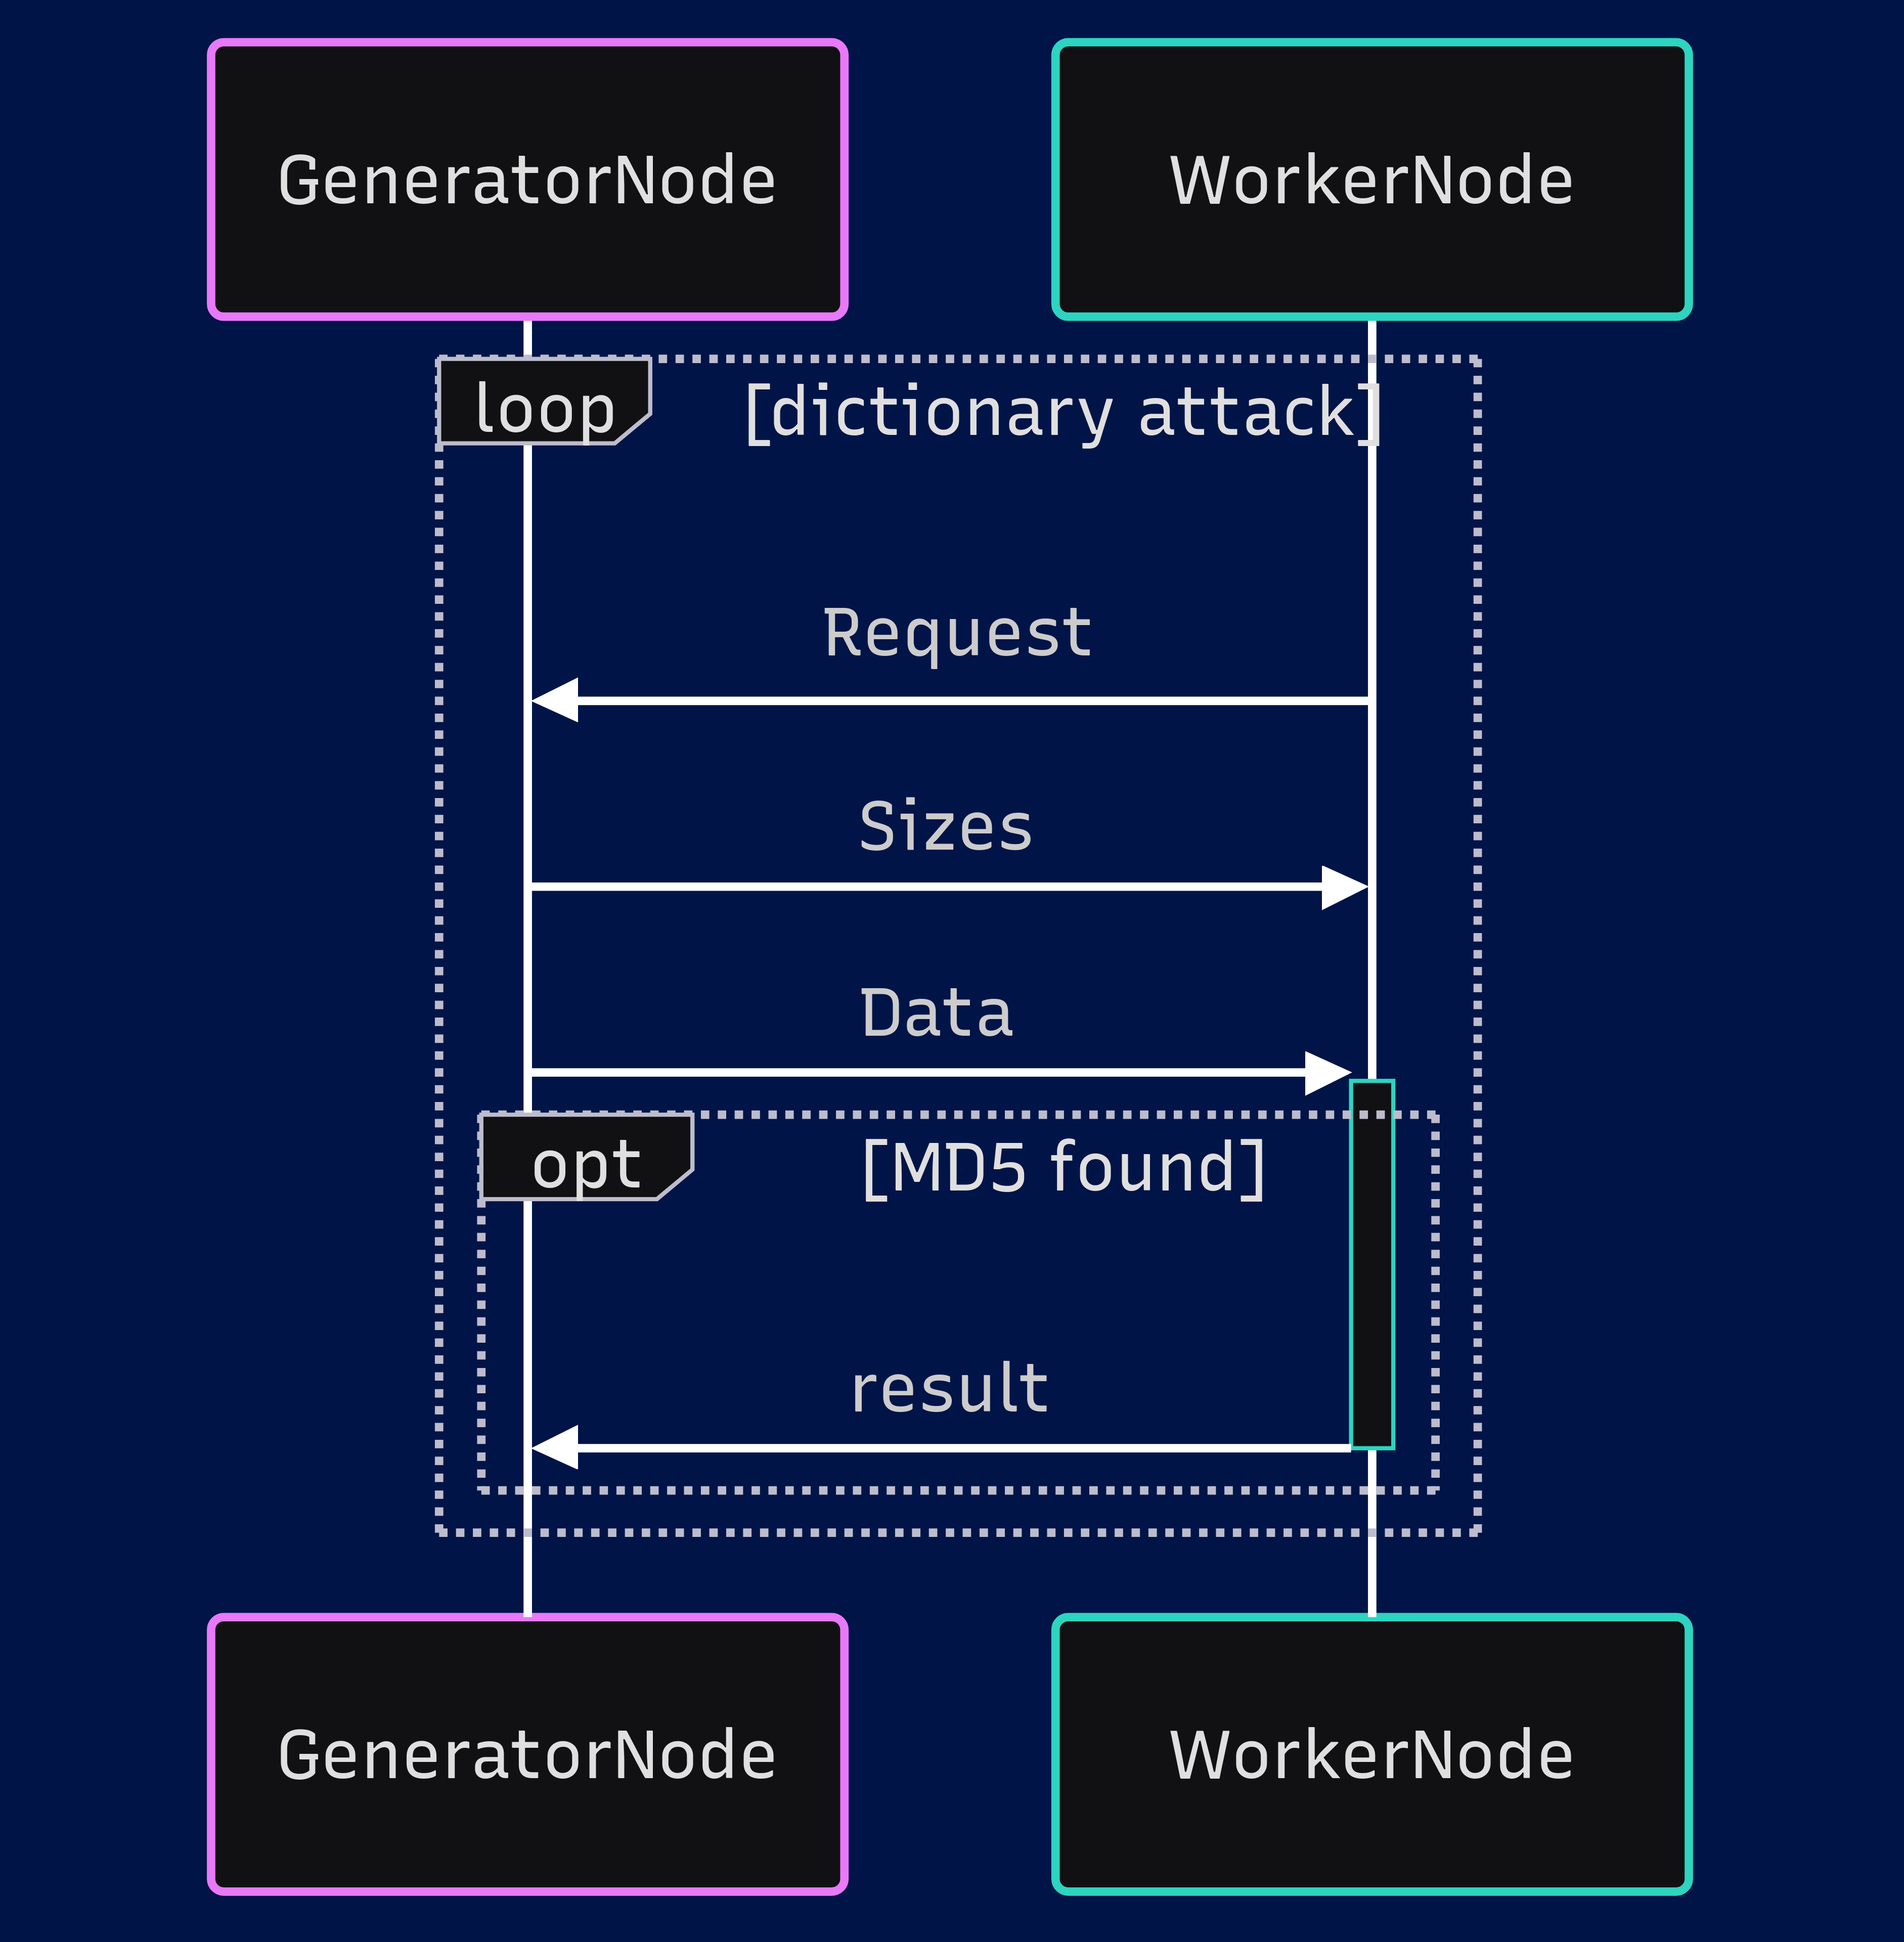
\includegraphics[width=0.5\textwidth]{images/chunk_workflow.png}
    \caption{Sequenze diagram of the chunked attack}    
\end{figure}

\subsubsection{The bruteforce attack}
In the bruteforce mode the communication needed is very tiny compared to the dictionary attack, also because a certain number of measure had been taken to prevent unnecessary movement of bytes, also between devices in the same computer. The message exchanged between the Generator and the Workers nodes is just a pair of integers that identify the span to be computed by a certain worker node, like in the previous case this communication is triggered by the worker that require a new task from the generator.



\printbibliography

\end{document}

